Dieses Kapitel befasst sich mit dem Konzept hinter der Implementierung, Dabei wird primär auf die Anforderungen der Netzwerkstruktur eingegangen.

\section{Anforderungen}
Es soll ein System geschaffen werden, welches das Spielen des Brettspiels \glqq{}Mensch Ärgere Dich Nicht\grqq{} für mindestens vier Spieler ermöglicht. Die Anforderungen an das System gliedern sich in zwei Teile: Anforderungen an das Spiel an sich, und Anforderungen an die unterliegende Netzwerkstruktur.\par

\subsection{Anforderungen -- Netzwerkstruktur}
Die Spieler sollen sich an verschiedenen Geräten, sowie in verschiedenen Subnetzen befinden können. Der zum Spielablauf notwendige Datenaustausch soll über ein \acs{WebRTC}-Peer-To-Peer Netzwerk zwischen den Spielern stattfinden. Dies setzt die Verwendung von STUN- und TURN-Servern vorraus. Es muss mindestens ein STUN- und ein TURN-Server existieren. Der Datenaustausch zwischen Peers muss dabei zuverlässig und geordnet sein.\par

Dritte sollen die STUN- und TURN-Server nur zu deren vorgesehenem Zweck -- zum Spielen des Brettspiels -- in Verbindung mit der Webanwendung nutzen können. Dazu müssen für jeden Nutzer dynamische, spezifische, zeitlich begrenzte Anmeldedaten erstellt werden, mit welchen eine Verbindung zu den Servern möglich ist. Diese Daten müssen beim Betreten eines Spiels an den jeweiligen Spieler vergeben werden.\par

\label{section:weitere}
Damit mehr als ein Spiel zur gleichen Zeit stattfinden kann, müssen die Spieler in Teilmengen unterteilt werden. Zwischen den Spielern in einer solchen Teilmenge müssen Signalisierungsdaten zum Verbindungsaufbau austauschbar sein. Spieler müssen diesen Teilmengen beitreten, und die Teilmengen verlassen können. Eine Teilmenge repräsentiert dabei einen virtuellen \glqq{}Tisch\grqq{} oder \glqq{}Raum\grqq{}. Ein \glqq{}Raum\grqq{} muss zudem über einen Spieler verfügen, welcher Berechtigungen zum Entfernen von Spielern besitzt, falls ein unerwünschter Spieler beitritt oder betrügt.\par

\subsection{Anforderungen -- Clientseitige WebRTC-Verbindungen}
Für jeden Peer muss ein Objekt existieren, welches sämtliche Verbindungen zu weiteren Peers verwaltet. Für jede Verbindung muss jeweils ein geordneter, zuverlässiger Datenkanal existieren. Es soll ein Event-Basiertes Nachrichtenprotokoll verwendet werden. Für verschiedene Events sollen -- ähnlich dem Syntax von Socket.io -- Rückruffunktionen registrierbar sein. Die Parameter dieser Rückruffunktionen sollen dabei die Daten des Events beinhalten.

\subsection{Anforderungen -- Brettspiel}
Um den Ablauf von Brettspielen zu beschreiben, und diesen als Zustandsmaschine darzustellen, werden hier einige Begriffe definiert, welche im Weiteren verwendet werden:

\begin{itemize}
    \item Ein \textit{Spieler} ist eine agierende Person, welche am Spiel teilnimmt. An einem Spiel nehmen stets $N$ ($1 \leq N \leq M$) Spieler teil. Im Falle des Spiels \textit{Mensch ärgere Dich nicht} gilt $M = 4 \geq N$.
    
    \item Eine \textit{Runde} ist ein Ablauf von $N$ \textit{Zügen}, wobei jeder      \textit{Spieler} je einmal \textit{am Zug} ist. War jeder Spieler je einmal am Zug, so wird eine neue Runde gestartet.
    
    \item Ein \textit{Zug} ist ein Ablauf an Aktionen eines Spielers. Der \textit{Zug} beginnt, wenn ein Spieler die Kontrolle über das Spiel zugewiesen bekommt. Der \textit{Zug} endet entweder, falls der Spieler aufgrund der Spielregeln keine valide Modifikation am Spielstand vornehmen darf, oder mit der Modifikation des Spielstands. Gewinnt der Spieler am Zug das Spiel, so wird dieser in den folgenden Runden übersprungen. Haben alle Spieler gewonnen, so wird das Spiel beendet. Falls nicht wird die Kontrolle an den nächsten Spieler übergeben, welcher dann wiederrum am Zug ist.
\end{itemize}

Das Brettspiel soll durch das einfache Aufrufen einer Website spielbar sein. Die Webanwendung soll das Spielen einer virtuellen Nachbildung des Gesellschaftsspiels \glqq{}Mensch Ärgere Dich Nicht\grqq{} ermöglichen. Das Spiel muss von bis zu vier Spielern gleichzeitig spielbar sein. Spieler sollen dem Spiel beitreten und es während das Spiel noch läuft wieder verlassen können. Falls beim Verlassen eines Spielers noch Spieler vorhanden sind, so sollen diese weiterspielen können. 

\subsubsection{Betrug}
In browserbasierten Webanwendungen ist es leicht, den JavaScript-Quellcode bei Laufzeit zu modifizieren. So können Spieler zum Beispiel unfaire Würfelergebnisse generieren, oder unerlaubte Spielzüge machen. Insbesondere die Würfelergebnisse lassen sich leicht manipulieren, ohne dass andere Spieler den Betrug überhaupt mitbekommen.\par

Spieler sollen daher nicht durch Modifikation von Script-Dateien betrügen können, ohne dass dies den anderen, nicht betrügenden Spielern angezeigt wird. Bei Benachrichtigung über den Betrug eines Spielers soll dieser Spieler vom, in Unterpunkt~\ref{section:weitere} beschriebenen, \glqq{}Host\grqq{}-Spieler aus dem Spiel entfernt werden können.\par

\subsubsection{Spielregeln}
Jeder Spieler besitzt vier Spielfiguren. Das Spiel wird auf einem Spielbrett gespielt. Auf diesem existieren jeweils 16 A-Felder, 16 B-Felder, sowie 40 weiße Felder. Dabei ist das erste Feld das gelbe, das zehnte Feld das grüne, das zwanzigste Feld das rote, und das dreißigste Feld das schwarze Startfeld (vgl. Abbildung~\ref{fig:maedngame}).\par 

\vspace{6pt}
\begin{figure}[h]
\centering
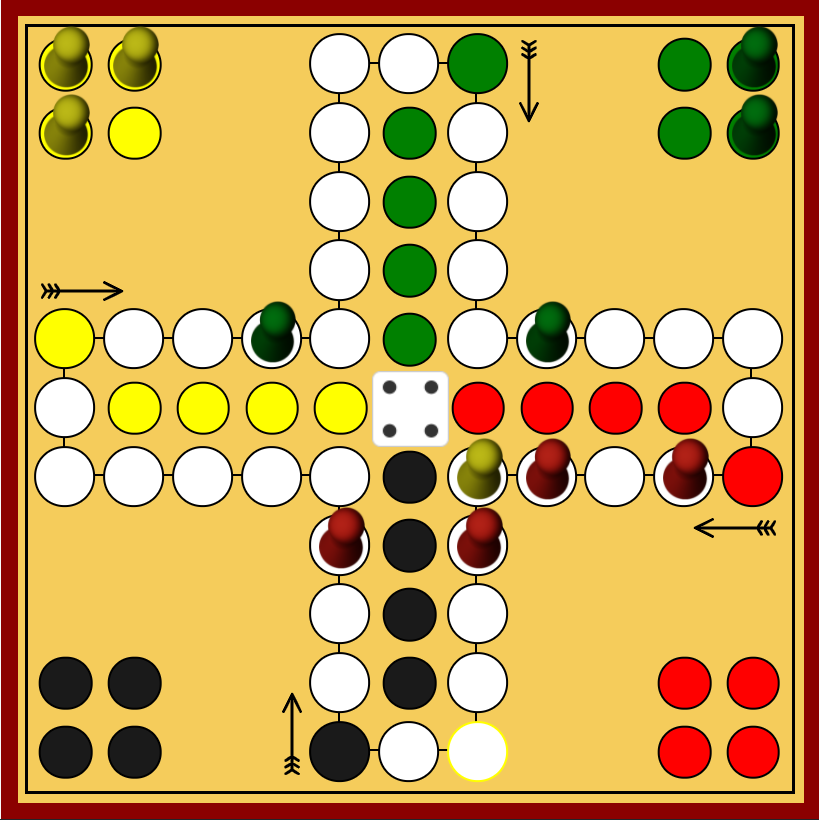
\includegraphics[width=0.75\textwidth]{bilder/game-in-progress.png}
\caption{Laufendes Spiel mit drei Spielern. Gelb ist am Zug. Die A-Felder sind die farbigen Felder am Rand des Spielbretts, die B-Felder sind die farbigen Felder in der Mitte des Spielbretts.}
\label{fig:maedngame}
\end{figure}

Bei Spielstart stehen alle Figuren auf den A-Feldern der jeweiligen Spieler. Ein Spieler hat gewonnen, wenn alle Figuren des Spielers auf dessen B-Feldern stehen. Das Spiel ist in Runden aufgeteilt, in jeder Runde ist jeder Spieler einmal am Zug. Jeder Spielzug beginnt mit dem Würfeln einer Zahl im Intervall [1,6]. Falls der Spieler eine sechs würfelt, so muss dieser, falls mindestens eine Figur in den A-Feldern ist, und das Startfeld des Spielers frei von eigenen Figuren ist, mit einer Figur die A-Felder verlassen. Die verlassende Figur wird auf das Startfeld des jeweiligen Spielers gestellt. Stehen alle Figuren eines Spielers bei Zugbeginn in den A-Feldern, so darf dieser bis zu drei mal würfeln, bis eine Sechs gewürfelt wurde. Würfelt ein Spieler eine Sechs, so darf dieser nach Wahl seines Spielzugs erneut würfeln. Nachdem ein Spieler seinen Zug beendet, ist der nächste Spieler im Uhrzeigersinn am Zug.\par

Landet eine Figur nach einem Spielzug auf einem Feld, wo bereits eine Figur eines anderen Spielers steht, so wird diese Figur \glqq{}geworfen\grqq{}, und muss in die A-Felder des Spielers zurück gesetzt werden.\par

Nachdem eine Figur -- relativ zum Startfeld eines Spielers -- 40 Felder weit bewegt wurde, kann diese die B-Felder eines Spielers betreten. In den B-Feldern dürfen Figuren nicht übereinander hinweg springen, und Würfe, welche die Figur über das letzte B-Feld hinaus bewegen würden, sind invalide. Nur der Spieler, welchem die B-Felder gehören, kann diese betreten.\par

Hat ein Spieler alle Figuren in dessen B-Felder bewegt, so können die weiteren Spieler das Spiel weiter zu Ende spielen. Gewonnene Spieler werden in Spielrunden ignoriert.\par

\section{Konzept -- Serverinfrastruktur}
Für die Raum-Funktionalität, Signalisierungsmechanismen, sowie die Generierung von STUN- und TURN-Anmeldedaten müssen entsprechende Server existieren. Für die Implementierung werden alle diese Funktionen prototypisch in einem Server zusammengefasst. Die konzipierte Netzwerkstruktur ist in Abbildung~\ref{fig:networkstructure} dargestellt. Neben der beschriebenen Signalisierungsebene müssen \acs{STUN}- und \acs{TURN}-Server gegeben sein. Beide diese Server sollen prototypisch in einem Server zusammengefasst sein. Dazu soll der \glqq{}coturn\grqq{} STUN- und TURN-Server verwendet werden.

\begin{figure}[h]
\centering
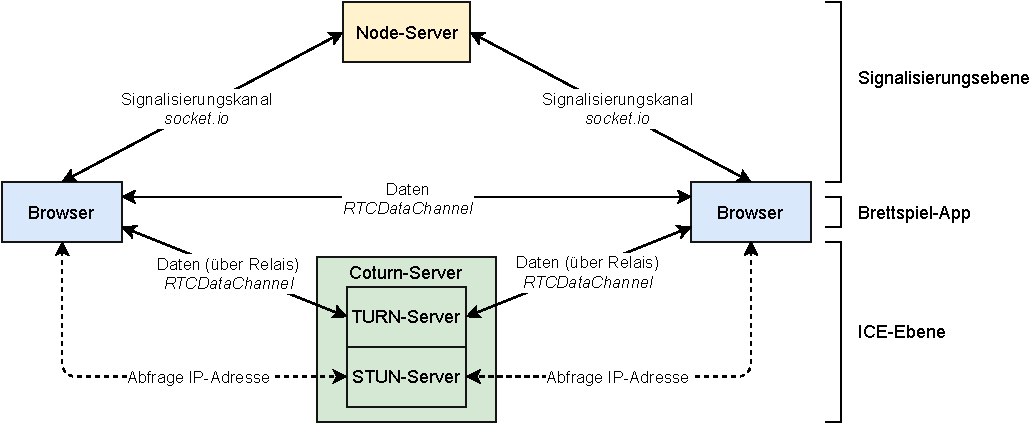
\includegraphics[width=0.95\textwidth]{bilder/PDF_SVG/NETWORK_STRUCTURE.pdf}
\caption{Konzept der Netzwerkinfrastruktur.}
\label{fig:networkstructure}
\end{figure}

\section{Konzept -- Peer-To-Peer Netzwerkarchitektur}
Bei der Netzwerkarchitektur des Peer-To-Peer Netzwerks kommen primär zwei Ansätze infrage: Das Authoritative-Peer-Modell, oder ein volles Peer-Netz.\par 

Das Authoritative-Peer-Modell folgt dem Authoritative-Server-Modell. Die Funktionen des Servers werden dabei von einem der Peers übernommen. Es wird eine Stern-Netzwerktopographie erzeugt, wobei der sogenannte \glqq{}Host-Peer\grqq{} den zentralen Knoten bildet. Bei $n$ Peers existieren insgesamt $n-1$ Verbindungen, der Host muss diese zu allen weiteren Peers aufrecht erhalten. Sämtlicher Datenaustausch läuft über den Host-Peer, welcher zudem die volle Authorität über den Spielstand besitzt. Die Client-Peers besitzen dabei nur den zur Darstellung des Spiels notwendigen, minimalen Spielstand. Der Vorteil dieses Modells ist die geringere Anzahl an Verbindungen im Netzwerk, sowie eine einfachere Entwicklung, da diese an das Authoritative-Server-Modell angelehnt werden kann. Problematisch ist jedoch der Single-Point-Of-Failure -- verliert der Host-Peer die Verbindung, so gehen alle Verbindungen sowie der Spielstand verloren. Für diese Fälle muss ein \glqq{}Host-Peer-Migrationsprozess\grqq{} existieren, um alle Verbindungen zu einem neu gewählten Host-Peer erneut zu erstellen. Existiert dieser nicht, so beendet das Verlassen des Host-Peers zwangsweise das Spiel.\par

Der Full-Mesh-Ansatz bildet das Gegenteil zum Authoritative-Peer-Modell. Hier verwaltet jeder Peer eine lokale Kopie des vollen Spielstands, und besitzt eine Verbindung zu jedem anderen Peer. Insgesamt existieren bei $n$ Peers also $n(n-1)$ Verbindungen im Netzwerk. Insbesondere bei hohen Datenraten und einer hohen Anzahl an Peers skaliert diese Netzwerktopologie schlecht, was jedoch in diesem Fall aufgrund der geringen Spieleranzahl, sowie des geringen Datenvolumens praktisch irrelevant ist. Letztendlich wurde dieser Ansatz für die Implementierung der Netzwerkarchitektur gewählt, da dieser keine komplexen Host-Migrationsprozesse vorraussetzt.\par

\section{Konzept -- Brettspiel}
Das Brettspiel soll via HTML5 und JavaScript im Browser implementiert werden. Die Darstellung des Spiels erfolgt mit stilisierten DOM-Elementen. Die Qualität der Darstellungs des Spiels ist hier nicht relevant, weshalb kein Frontend-Framework verwendet wird.\par

\subsection{Zufallszahlen}
Ist die Netzwerktopographie eines Brettspiels ein Authoritative-Server-Modell, so ist es leicht, faire und unabhängige Zufallszahlen zu erstellen. Ein Client kann einfach eine Anfrage an den Server schicken, welcher eine Zahl generiert und an den Client zurückschickt. Macht der Spieler darauf einen Spielzug, so kann dieser vom Server mit Hinblick auf die zuvor generierte Zufallszahl validiert werden. In einem Full-Mesh Peer-Netzwerk ist dies nicht ohne weiteres möglich \cite{rng}.\par

\subsubsection{Verteiltes Generieren von Zufallszahlen}
Ein naiver Ansatz zur Generation von Zufallszahlen ist, jeden Peer $n$ eine Zahl $z_n$ bis zu einem Wert $max$ generieren zu lassen, welche zwischen den Peers ausgetauscht werden. Anschließend ergibt die folgende Summe bei $n$ Peers eine Zahl, welche -- vorrausgesetzt mindestens einer der Peers hat eine zufällige Zahl generiert und nicht betrogen \cite{rng} -- zufällig ist:

\vspace{-20pt}
\[ z = \sum_{n=1}^{n} z_n \mod n,\quad z, z_n \in [0, max] \]
\vspace{-12pt}

Hier existiert jedoch das sogenannte \glqq{}Look-Ahead-Problem\grqq{}, wobei ein Peer einfach auf die Zufallszahlen aller anderen Peers warten kann, bevor dieser die eigene Zufallszahl abgeschickt hat. Basierend auf den Zufallszahlen der weiteren Peers kann der böswillige Peer nun eine Zahl abschicken, welche diesem ein gewünschtes Ergebnis -- verbunden mit einem Spielerischen Vorteil -- bringt. Für dieses Problem existieren Lösungsansätze wie das \glqq{}Lockstep-Protokoll\grqq{} \cite{p2pchallenges}, unter Nutzung von Commitment-Verfahren \cite{rng}. Bei einem Commitment-Verfahren werden die zu sendenden Daten zuerst mit einem Passwort verschlüsselt und unter den Teilnehmern ausgetauscht. Sind alle verschlüsselten Daten ausgetauscht, so werden die Passwörter ausgetauscht. Es ist einem Peer somit nicht ohne weiteres möglich, auf alle weiteren Zahlen zu warten, ohne vorher eine eigene Zahl erstellt zu haben \cite{rng}.\par

\subsubsection{Seeded Random-Number-Generators}
Eine andere Methode zur Generierung von fairen Zufallszahlen in verteilten Systemen wie Peer-Netzwerken sind \glqq{}Seeded-Random-Number-Generators\grqq{}  \cite{rng}\footnote{vgl. Sektion 1.2 und verwandte Werke}. Dabei lässt sich ein Zufallszahlengenerator mit einem Startwert, dem sogenannten \glqq{}Seed\grqq{}, initialisieren. Der Generator erzeugt basierend auf diesem Seed eine Folge an Pseudozufallszahlen, welche unter Nutzung des gleichen Seeds stets gleich ist. Um eine hinreichende Zufälligkeit der Zahlenfolge zu garantieren, ist der Seed in der Regel eine Zufallszahl, welche zum Beispiel einmalig von einem Server generiert werden kann. Besitzt jeder Peer den gleichen Seed, so muss nur die Aktion des Generierens an sich synchronisiert werden -- daraufhin generiert jeder Peer eine faire, unabhängige Pseudozufallszahl. Wichtig ist hierbei, dass der Spielstand zwischen den Peers unbedingt synchron gehalten werden muss. Generiert ein Teilnehmer eine Zahl zu viel oder zu wenig, so sind die Generatoren nicht mehr synchron. Dieser Ansatz bietet sich bei Brettspielen besonders an, da diese -- im Gegensatz zu Echtzeitspielen -- in der Regel in klar definierte \glqq{}Züge\grqq{} und \glqq{}Runden\grqq{} eingeteilt sind. Ein synchroner Spielstand zwischen den Spielern ist somit einfach beizubehalten. Aus diesem Grund wurde dieser Ansatz für die Implementierung gewählt.\par

